\documentclass{article}
\usepackage[utf8]{inputenc}

\title{Cosmological Evidences of Dark Matter through the CMB}
\author{Lorenzo Speri}
\date{}
\usepackage{hyperref}
\usepackage{natbib}
\usepackage{graphicx}
% ---- Maths -------
\usepackage{amsmath}
\usepackage{amsthm}
% ---- Links -------
\usepackage{hyperref}

%  ---- my commands -------
\newcommand{\bea}{\setlength{\jot}{10pt}\begin{eqnarray*}}
\newcommand{\eea}{\end{eqnarray*}}
\newcommand{\beq}{\begin{equation}}
\newcommand{\eeq}{\end{equation}}
\newcommand{\bpsi}{\bar{\psi}}
\newcommand{\dslash}{\slashed{\partial}}
\newcommand{\Dslash}{\slashed{D}}
\newcommand{\Lagr}{\mathcal{L}}
\newcommand{\cpp}{\texttt{C++} } 
\newcommand{\mpi}{\texttt{MPI} } 
\newcommand{\de}{\nu}
\newcommand{\T}{\text{TT}}
\newcommand{\h}{\mathscr{H}}
\newcommand{\ten}{\mathscr{T}}

\begin{document}

\maketitle


\section{Introduction}
Many astronomical and cosmological observations suggest that there is a missing form of matter that interacts gravitationally. 
In order to explain such observations, scientists have proposed the existence of Dark Matter, a new form of matter that does not interact electromagnetically but gravitationally.
However, the fundamental nature of Dark Matter is not well understood yet, and whether Dark Matter is truly a new form of matter or the effect of new laws of gravity is still matter of debate.\\
One of the most compelling evidence for the existence of Dark Matter comes from the analysis of the Cosmic Microwave Background (CMB).
In this paper we explain how the  analysis of the CMB is linked to the energy-matter content of our Universe, and, within this framework, we study the role of Dark Matter.
The aim of this paper is to give a short and concise overview of the cosmological evidence of Dark Matter given by the observations of the CMB.
\\


The Cosmic Microwave Background is the electromagnetic radiation coming from the hot plasma of the early stages of the Universe.
When the Universe, made of hot plasma, reached a temperature low enough to form stable hydrogen $e^- + p^+  \rightarrow H + \gamma$ the number density of the free electrons dropped, causing the Thomson scattering $e^- + \gamma  \rightarrow e^- + \gamma$ to be inefficient and the photons to decouple. They have since streamed freely through the universe and are today observed as the Cosmic Microwave Background \citep{LecturesPdf}.\\
 
 

\subsection{to be put in the paper or at the end}
-practical Motivation for studyinbg the cmb: nice spectrum black body spectrum: physics well know, very intense radiation\\
which info can we get from the cmb: Big bang, maater and energy content of the universe---dark matter is a big part of the matter content it influenced the spectrum  of the CMB ---- so it played a role.\\
-structure of the paper \\



%The recent measurements of the Cosmic Microwave Background (CMB) radiation allowed us to infer the presence of Dark Matter in the Universe. In this summary we will explain qualitatively how the presence of Dark Matter influences the CMB anisotropies.

\section{From the Discovery of the CMB to the Planck mission}

\begin{figure}
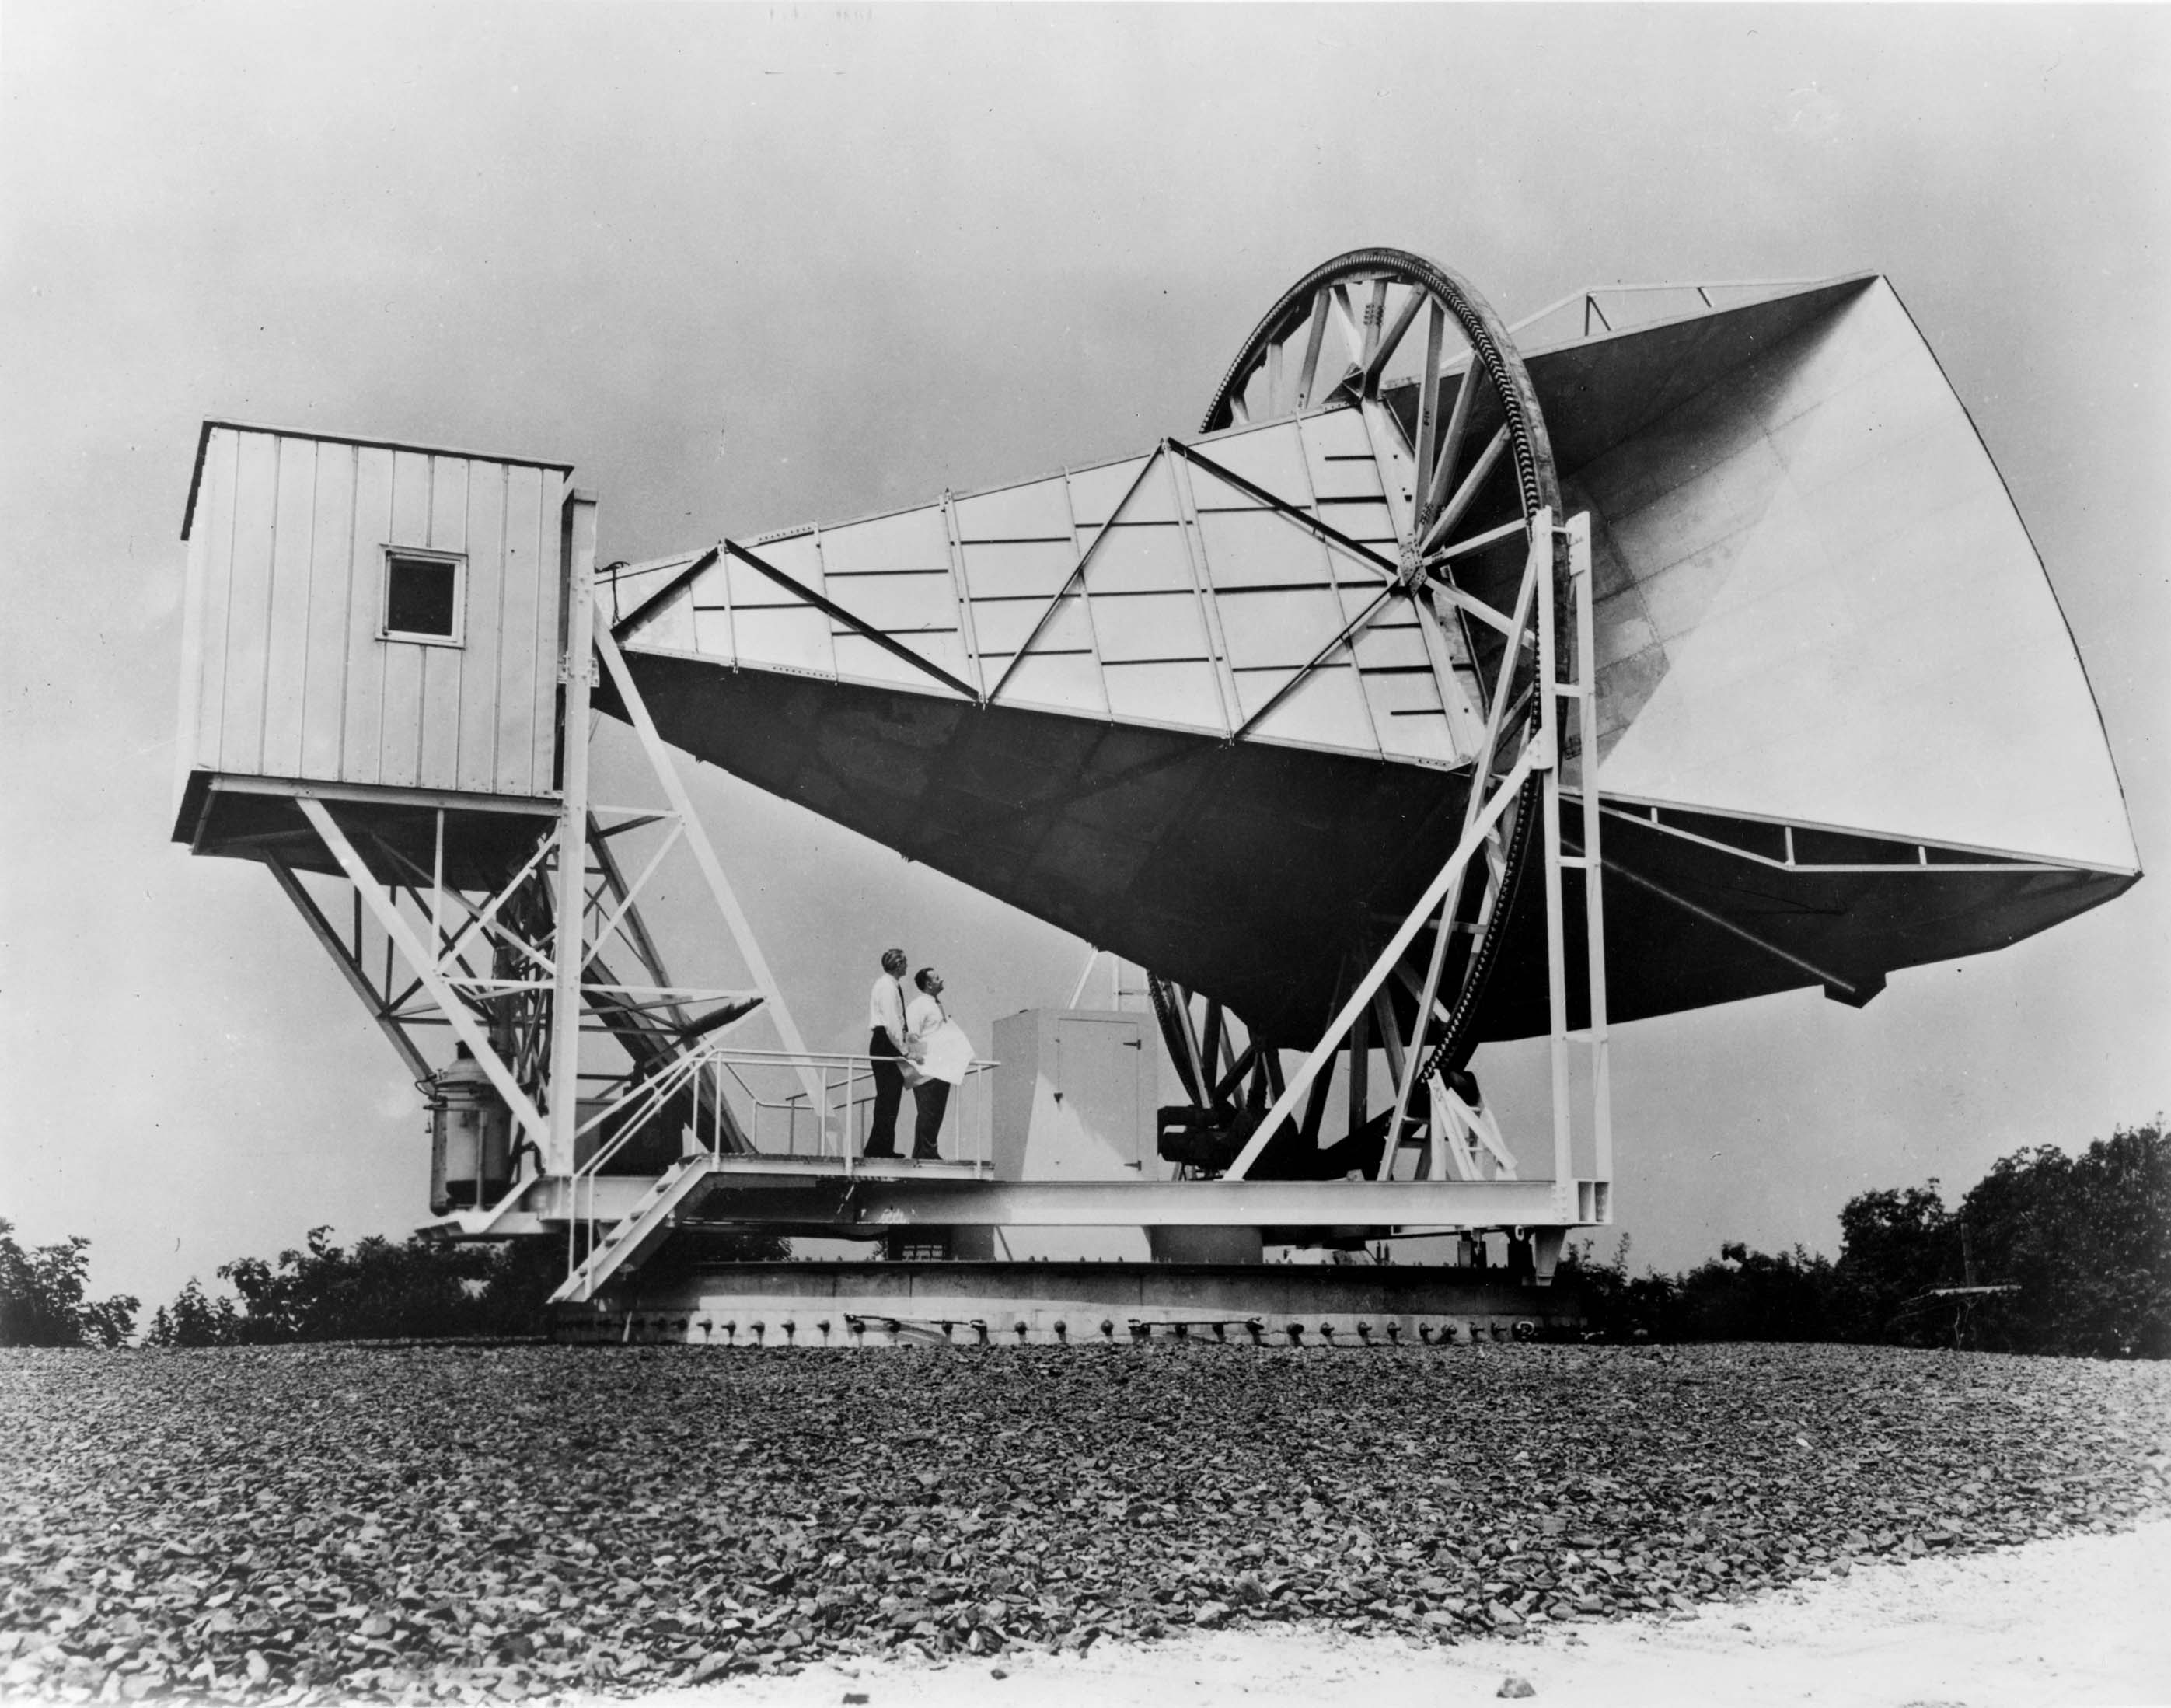
\includegraphics[width=\textwidth]{Horn_Antenna.jpeg}
\caption{The 15 meter Holmdel horn antenna at Bell Telephone Laboratories in Holmdel, New Jersey.
(By NASA - Great Images in NASA Description, Public Domain, \url{https://commons.wikimedia.org/w/index.php?curid=6463768})}
\end{figure}

In 1965 Arno Penzias and Robert Wilson published the paper: \emph{A measurement of excess antenna temperature at
4080 Mc/s}, where they reported the measurements of an isotropic, unpolarized, and free from seasonal variations excess noise temperature
\citep{penziasMeasurementExcessAntenna1965}. 
When Penzias and Wilson first measured serendipitously this strong signal, they did everything they could think of to reduce “noise” in their system. 
They even shooed away a pair of pigeons that had roosted in the antenna and cleaned up they later called “the usual white dielectric” generated by pigeons \citep{RydenIntroCosmoPdf}.
However, the signal remained. 
Robert Dicke and his research group at Princeton University explained such signal as the relic of an early, hot, dense, and opaque state of the universe\footnote{the existence of the cosmic background radiation had actually been predicted by the physicist George Gamow and his colleagues in 1948} \citep{bucherPhysicsCosmicMicrowave2015}
. \\
This discovery of the CMB created a big excitement and a new era of cosmology began.
Measuring the CMB spectrum and its deviation from the black body spectrum was the new challange.
Many experimental efforts have been carried out to measure accurately the fluctuations of Cosmic Microwave Backgrund from its average temperature $T = 2.7$ K, we will discuss only few of them.
\\
First of all, the photons of the CMB can be absorbed by the Earth's atmosphere, because the energy per CMB photon (approximately $\sim 6 \times 10 ^{-4}$ eV) is comparable to the energy of vibration or rotation for a small molecule (of water for instance). In fact, microwaves with wavelengths shorter than $\lambda \sim 3$ cm are strongly absorbed by water molecules \citep{RydenIntroCosmoPdf}.
This problem could be overcomed by observing the CMB in different bands and from locations where the humidity is low.
However, the best way to meseaure the CMB spectrum is to use satellites.\\
The first sattellite that was launched to observe the CMB was COBE. 
It did provide a convincing first detection of the CMB anisotropy, and it played a crucial role in determining the viability of the different cosmological models at that time.
\\
After that, WMAP and PLanck space missions  increased the accuracy of the measurements Figure (\ref{cobe_wmap_planck}).
Nevertheless the satellites improved their accuracy, many other sources of noise were encountered such as the light coming from the center of our galaxy, other stars and other objects in the universe, in addition to the relative motion of the satellite with respect to the CMB (Figure (\ref{cobe_map})).\\
Finally, observations and statistical analysis showed that the CMB spectrum is close to a black body spectrum up to fluctuations of order of $10^{-5}$ K (Figure (\ref{cobe_blackbody})).\\
% maybe last sentence in the introduction with the image


\begin{figure}
\centering
    \textbf{CMB spectrum}\par\medskip
\centering
   {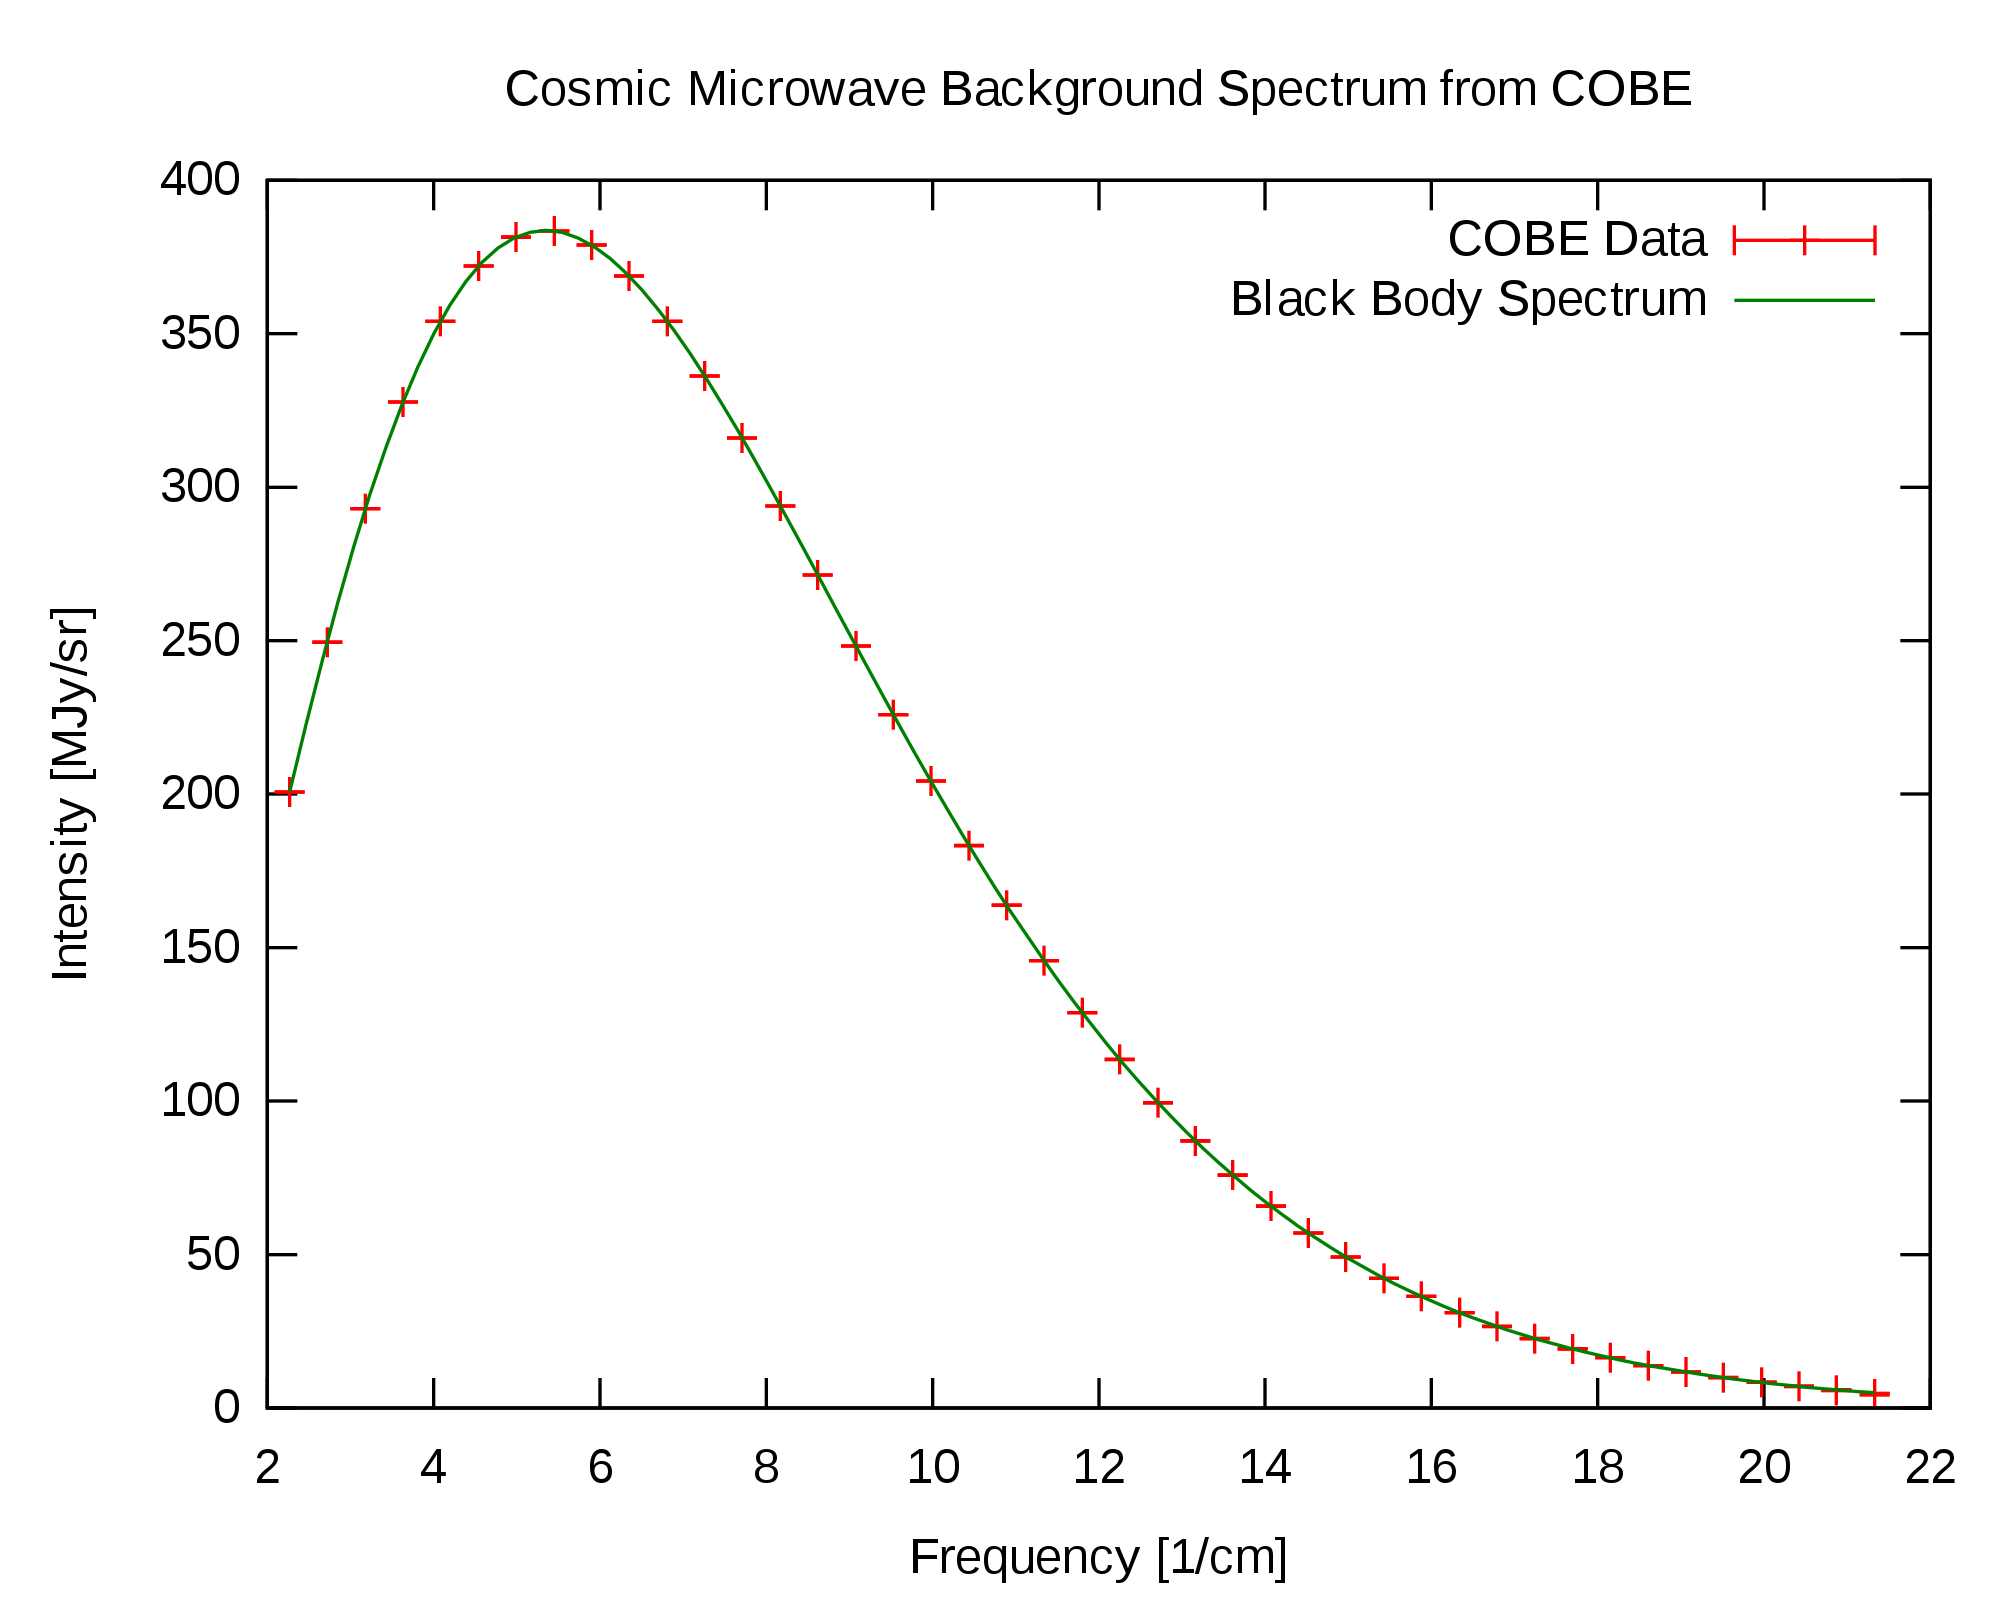
\includegraphics[height=8cm]{blackbody.png}}
\caption{}
\label{cobe_blackbody}
\end{figure}


\begin{figure}
\centering
    \textbf{The Cosmic Microwave Background anisotropies measured by COBE, WMAP and Planck}\par\medskip
\centering
   {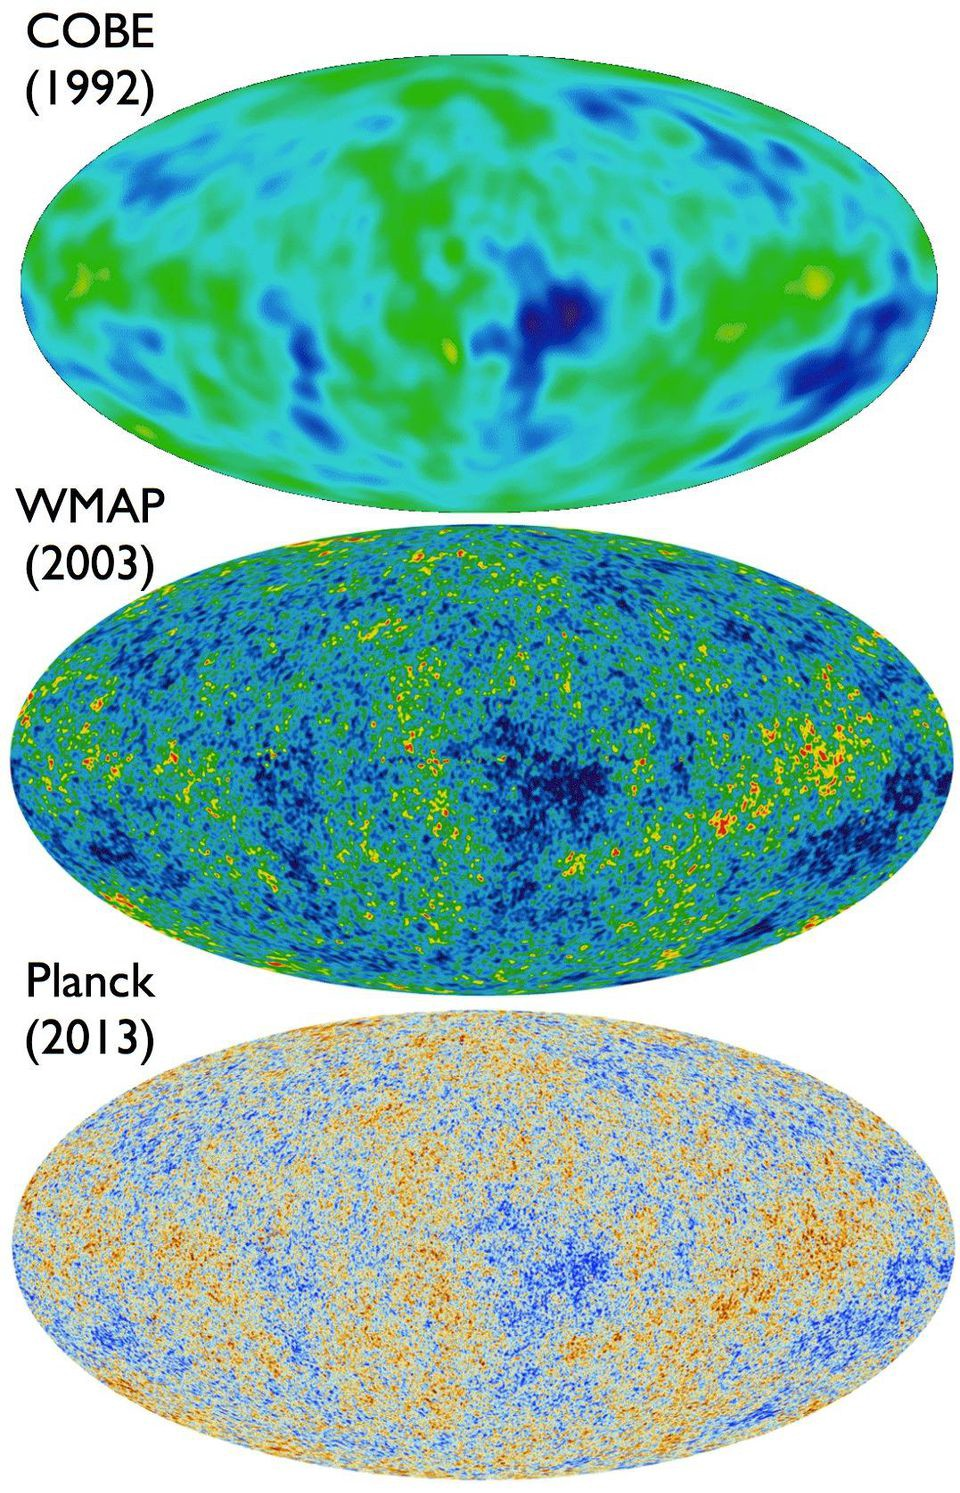
\includegraphics[width=.45\textwidth]{cobe_wmap_planck.jpg}}


\caption{The COBE, WMAP and Planck missions measured the CMB anisotropies with increasing accuracy. COBE, the first CMB satellite, measured fluctuations to scales of 7$^\circ$. WMAP was able to measure resolutions down to 0.3$^\circ$ in five different frequency bands, with Planck measuring all the way down to just 5 arcminutes (0.07$^\circ$) in nine different frequency bands in total.  (NASA/COBE/DMR; NASA/WMAP SCIENCE TEAM; ESA AND THE PLANCK COLLABORATION)}
\label{cobe_wmap_planck}
\end{figure}


\begin{figure}
\centering
    \textbf{Orbits of different  configurations of BBH}\par\medskip
\centering
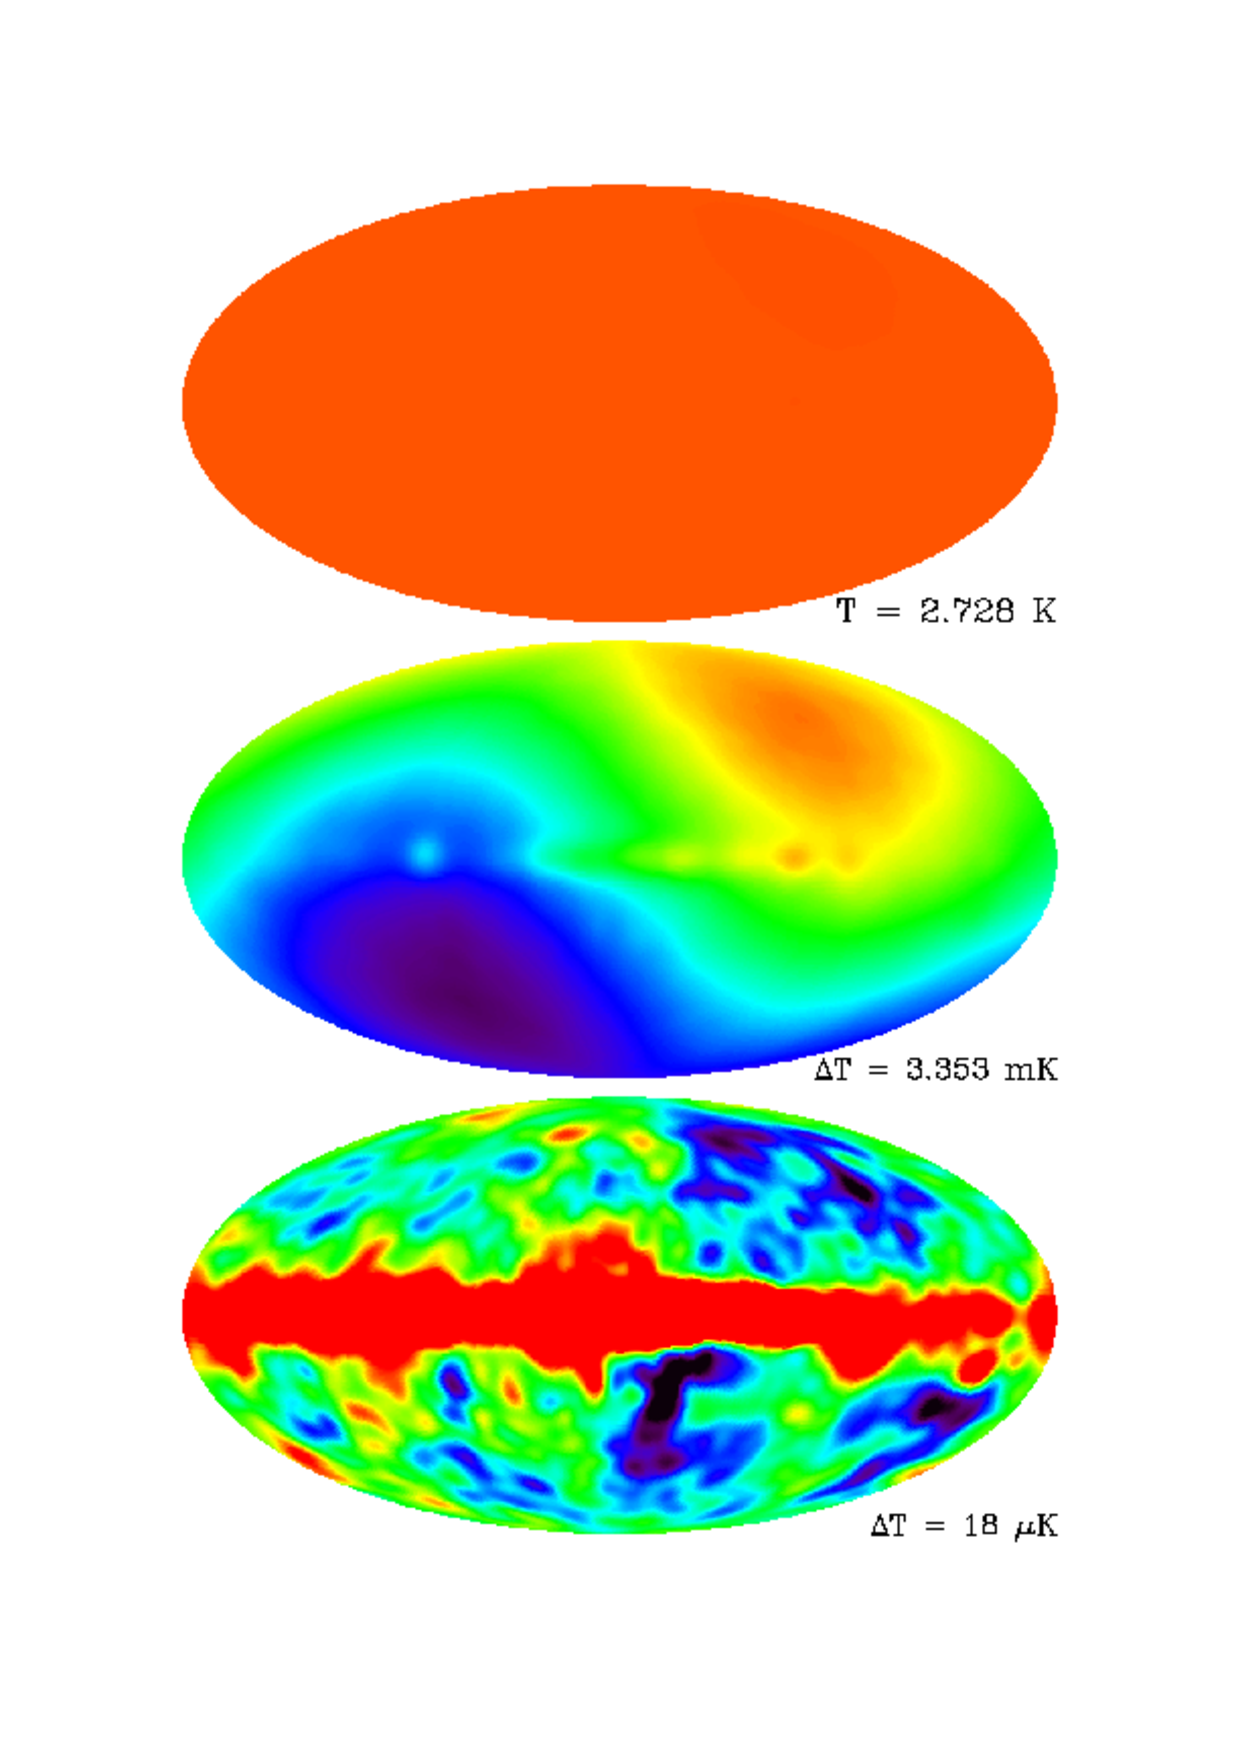
\includegraphics[scale =0.3]{mono_di_cobe}
\caption{The microwave sky as seen by the COBE DMR (differential microwave radiometer) instrument. The top panel shows the microwave sky as seen on a linear tem- perature scale including zero. No anisotropies are visible in this image, because the CMB monopole at 2.725K dominates. In the middle panel, the monopole component has been subtracted. Apart from some slight contamination from the galaxy near the equator (corre- sponding to the plane of our Galaxy), one sees only a nearly perfect dipole pattern, owing to our peculiar motion with respect to the rest frame defined by the CMB. In the bottom panel, both the monopole and dipole components have been removed. Except for the galactic contamination around the equator, one sees the cosmic microwave background anisotropy along with some noise. (Credit: NASA/COBE Science Team)}
\label{cobe_map}
\end{figure}

\section{Content of the Universe}
The General Theory of Relativity is the best theory of gravity that we have, so far. So,  
\begin{itemize}
\item Assumptions: working with the $\Lambda$CDM model
\item General relativty
\item Friedmann equations
\end{itemize}

\section{CMB theo analysis}
\begin{itemize}
\item hydrodynamics \citep{huLectureNotesCMB2008}
page 14 eq 49 to page 17 eq 71\\
skip doppler effect
\item gravito acoustic oscillations page 19 up to eq 82 , justify briefly constant potential in page 20
% if stress perturbations are negligible compared with density perturbations ( δp ≪ δρ ) then the potential will remain constant in periods where the background equation of state p/ρ is constant
\item page 20 and 21 up to eq92 important comment 
%The consequence is that overdense regions where Ψ is negative (potential wells) are cold spots in the effective temperature.
\item baryonic effect
\end{itemize}

\section{Comments on the results and plots of the CMB spectrum}







\section{Conclusion}
nn
\citep{padmanabhanDetectingDarkMatter2005}



\bibliographystyle{plain}
\bibliography{dark_1}
\end{document}
